\documentclass[12pt, titlepage]{article}

\usepackage{booktabs}
\usepackage{tabularx}
\usepackage{hyperref}
\hypersetup{
    colorlinks,
    citecolor=black,
    filecolor=black,
    linkcolor=red,
    urlcolor=blue
}
\usepackage[round]{natbib}
\usepackage{enumitem}
\usepackage{float}
\usepackage{amsmath}
\usepackage{tikz}
\usepackage[normalem]{ulem}
\usepackage{xcolor}
\usetikzlibrary{automata,positioning,arrows}
\usepackage{lscape} 

\newcommand\redsout{\bgroup\markoverwith{\textcolor{red}{\rule[0.5ex]{2pt}{0.4pt}}}\ULon}

\title{SE 4G06: Software Requirements Specification\\Team \#12 - CodeChamp}

\author{
  Kanugalawattage, Anton
  \and
  Subedi, Dipendra
  \and
  Rizkalla, Youssef
  \and
  Leung, Tamas
  \and
  Zhao, Zhiming
}


\date{\today}

\input{../Common}
\input{../Comments}

\begin{document}

\maketitle

\pagenumbering{roman}

\begin{table}[h]
\caption{\bf Revision History}
\begin{tabularx}{\textwidth}{p{3cm}p{2cm}X}
\toprule {\bf Date} & {\bf Version} & {\bf Notes}\\
\midrule
Mar. 30, 2023& 0.4 & Updated non functional requirements with fit criterion, Added context diagram, off the shelf solutions. Reformatted multiple sections. Added additional terminology. Fixed tractability matrix. Updated requirements priority and reasoning. Updated user state diagram\\
Feb. 7, 2023& 0.3 & Updated Functional and Non functional requirements\\
Oct. 4, 2022 & 0.2 & Prioritization, Traceability and Phase In Plan for Requirements; Appendix Reflections; Minor changes to requirements; State Machine Formal definition\\
Sept. 27, 2022 & 0.1 & Initial Version\\
\bottomrule
\end{tabularx}
\end{table}

\newpage

\tableofcontents
\listoftables
\listoffigures

\newpage


\section*{Document Template}
The following document follows the Volere Simplified Template, which is described  \href{https://gitlab.cas.mcmaster.ca/smiths/se3xa3/tree/master/BlankProjectTemplate/Doc/SRS}{here}. In addition, some sections were added. Primarily, a section was added to describe the Phase-in Plan to plan a schedule for the engineering team in regards to the development of important functional requirements. Additionally, requirements were given priorities which are described in their respective section to be prioritized by the team. Finally, a traceability table was given to describe the relationship between the functional and non-functional requirements.


\section*{Naming Conventions and Terminology}
\begin{table}[H]
\begin{center}
\begin{tabular}{|p{3cm}|p{9cm}|}
\hline
  \textbf{Symbol} & \textbf{Description}\\
  \hline
  Data Structures and Algorithms & A topic of study for Computer Scientists.\\
  \hline
  CodeChamp & The system being built.\\
  \hline
  Client & A device used to connect to a CodeChamp instance.\\
  \hline
  DSA & Abbreviation for Data Structures and Algorithms.\\
  \hline
  UI & Abbreviation for User Interface.\\
  \hline
  SRS & Abbreviation for Software Requirements Specification.\\
  \hline
  Coding Problem & A problem in which user has to write code which optimally solves a described problem. Also sometimes referred to as an algorithmic problem.\\
  \hline
  \href{http://www.leetcode.com}{LeetCode} \cite{leetcode} & An online platform to learn data structures and algorithms. It provides the user with the ability to solve questions from the database by giving them the ability to write code and compile within the platform.\\
  \hline
  \href{https://codeforces.com/}{CodeForces} \cite{codeforces} & Another online platform to learn data structures and algorithms.\\
  \hline
  Match & A game set between multiple users, usually divided into multiple rounds.\\
  \hline
  Round & An instance of a game in which some players either win the match or qualify for another round. The remainder of the players are eliminated from the match.\\
  \hline
  Matchmaking & The process of finding users to play a game against or with each other.\\
  \hline
  Lobby & A staging area which multiple users can join before playing a game.\\
  \hline
  Match History & A section commonly found in online games which allows users to see the results of matches they have recently played in.\\
  \hline
\end{tabular}
\end{center}
\caption{Symbols, Abbreviations and Acronyms}            

\end{table}
\newpage

\pagenumbering{arabic}

% This document describes the requirements for ....  The template for the Software
% Requirements Specification (SRS) is a subset of the Volere
% template~\citep{RobertsonAndRobertson2012}.  If you make further modifications
% to the template, you should explicity state what modifications were made.



\section{Project Drivers}

This section details the motivation behind the project, identifies potential stakeholders and describes the constraints around the CodeChamp system. Additionally, it states assumptions about the intended audience of the system.

\subsection{The Purpose of the Project}

Practicing coding the traditional way can be daunting. The current most popular method to learn is to use a problem database site like \href{http://www.leetcode.com}{LeetCode} \cite{leetcode}. This method of learning can often feel tiring and endless. There are over 2000 problems on the website which can be intimidating to many new coders. CodeChamp will introduce a collaborative and fun way to interact with your friends while improving your algorithmic skills.

\subsection{The Stakeholders}

\subsubsection{The Client}
The main clients for this project are Dr.Spencer Smith and the TAs of SE 4G06. They oversee and supervise the development of CodeChamp through providing feedback and suggestions.

\subsubsection{The Customers}
The main customers of CodeChamp are learners who wants to practice and improve on their data structures \& algorithmic skills. CodeChamp provides tools for learners to practice on many different algorithmic problems. CodeChamp will be an effective alternative to existing users of popular coding practice sites like LeetCode and CodeForces. Additional customers of CodeChamp are players who want to compete or play against other players in CodeChamp. CodeChamp provides gaming experience for players to code in a multiplayer experience.

\subsubsection{Other Stakeholders}
Additional stakeholders for CodeChamp is the development team of CodeChamp. They decide on the requirements and design of the system and seek feedback from other stakeholders to improve CodeChamp.

\subsection{Mandated Constraints}

\subsubsection{Solution Constraints}
The system shall be accessible through the internet to any device with a
browser.

\subsubsection{Budget Constraints}
For the scope of the project, deployment and hosting shall cost less than \$750

\subsection{Relevant Facts and Assumptions}
CodeChamp assumes users will maintain a steady internet connection throughout the game, and already understands how to input on a browser. CodeChamp is built for users who are able to handle stable internet communication and understand how web browser interfaces work. The assumed method of input for users are keyboard and mouse. Other methods of input are not considered due to the lack of support in modern browsers.

\section{Functional Requirements}

This section details the functional requirements of CodeChamps systems. Primarily, it describes the context of the product and the product's use cases. Moreover, the functional requirements are given and prioritized. Additionally, a state machine is given to described the intended flow for the CodeChamp experience. Finally, a phase in plan is described for the functional requirements.

\subsection{The Scope of the Work and the Product}

\subsubsection{The Context of the Work}
\begin{figure}[H]
    \hspace{-3cm}
    \includegraphics{context_diagram.pdf}
    \caption{Context Diagram for the CodeChamp System}
    \label{fig:context-diagram}
\end{figure}

\subsubsection{Work Partitioning}
The servers will handle all match data, compile user's submissions and evaluate the correctness of user submissions. The user's client interface will request match data and match state from server and communicate with server to update match status.

\subsubsection{Individual Product Use Cases}
The following diagrams describes the product use cases for the users:

\begin{figure}[H]
    \includegraphics{usecasediagram.pdf}
    \caption{Use Case Diagram for CodeChamp}
    \label{fig:context-diagram}
\end{figure}


\subsection{Functional Requirements}
\subsubsection{Priority 0}
\begin{enumerate}[label=FR.\arabic*]
    \item The system shall match-make users into a lobby. \label{FR.1}
    \item The system shall allow the user to be start the game whenever there is one or more player in a lobby. \label{FR.2}
    \item The system shall allow for multiple rounds in a match. \label{FR.3}
    \item The system shall display one coding problem per round. \label{FR.4}
    \item The system shall allow users to submit code through the web interface. \label{FR.5}
    \item The system shall compile the user's code. \label{FR.6}
    \item The system shall run the user's code against the test cases for a problem.  \label{FR.7}
    \item The system shall display the result of running the submitted code against the test cases to the user.  \label{FR.8}
    \item The system shall allow for players to be eliminated.  \label{FR.9}
    \item The system shall only allow for one winner in each match. \label{FR.10}
    \item The system shall allow developers to create, modify and delete coding problems.  \label{FR.11}
    \item The system shall allow developers to create, modify and delete test cases for a coding problem. \label{FR.12}

\end{enumerate}

\subsubsection{Priority 1}
\begin{enumerate}[label=FR.\arabic*, resume] 
    \item The system shall allow users to log in. \label{FR.13}
    \item The system shall display an error if the user fails to log in. \label{FR.14}
    \item The system shall track the code's running time in seconds and its memory usage in megabytes. \label{FR.15}\\
    \textbf{Rationale}: An important part of an algorithm is its time and memory complexity. For some problems, the developers may want to disallow solutions that are not of the optimal time or memory complexity.
    \item The system shall time-out any code that exceeds the time or memory limit for a coding problem. \label{FR.16} \\
     \textbf{Rationale}: Inputs that consume more resources than needed should be timed out for performance and safety of the system.  
    \item The system shall allow developers to define a time in seconds and a memory limit in megabytes for each coding problem. \label{FR.17}

\end{enumerate}

\subsubsection{Priority 2}
\begin{enumerate}[label=FR.\arabic*, resume]
    \item The system shall allow users to create a lobby link. \label{FR.18}\\
     \textbf{Rationale}: Links will be used to allow users to share a lobby to other users.
    \item The system shall allow users to join a lobby using a link. \label{FR.19}\\
      \textbf{Rationale}: With the links created, users should be able to join lobbies.=
    \item The system shall allow users to view a history of their previous matches. \label{FR.20}
     \textbf{Rationale}: Allows the user to see their history and progress to track their skill changes over time.
    \item The system shall display the user's win percentage. \label{FR.21}\\
     \textbf{Rationale}: Allows the user to track their history and progress to quantify their skills against the competition.
    \item The system shall display what placement they received in the match history. \\
    \textbf{Rationale}: Looking at a previous matches' result is helpful for the user experience, as it can help them recognize what they did wrong and what they could do to improve in the next one.
    \label{FR.22}
    \item The system shall display the coding problem for each round in a match's history.\\
    \textbf{Rationale}: Looking at previous problems can help users identify their weaknesses and give them a second chance to solve a problem which they could not previously solve in time. \label{FR.23}
    \item The system shall track and display the top 100 users with the largest number of wins. \label{FR.24}\\
    \textbf{Rationale}: Recognizing the top users can motivate others to practice and give an incentive for improvement, which is important for our user experience. 

\end{enumerate}

\subsection{User State Finite State Machine}
The following state diagram shows the possible states a user can be in. State s\_login is the state where the user must login before being able to use the system. State s\_idle is where the user is not in a game or a lobby. State s\_lobby represents the state in which users are waiting for other players to join. State s\_ingame represents the state in which users are in a game. State s\_endscreen represents the state where the user has completed the game and is shown their result.

%% Machine generated by https://finsm.io
%% 2022-9-27-20:08:038
\begin{figure}[H]
    \centering
    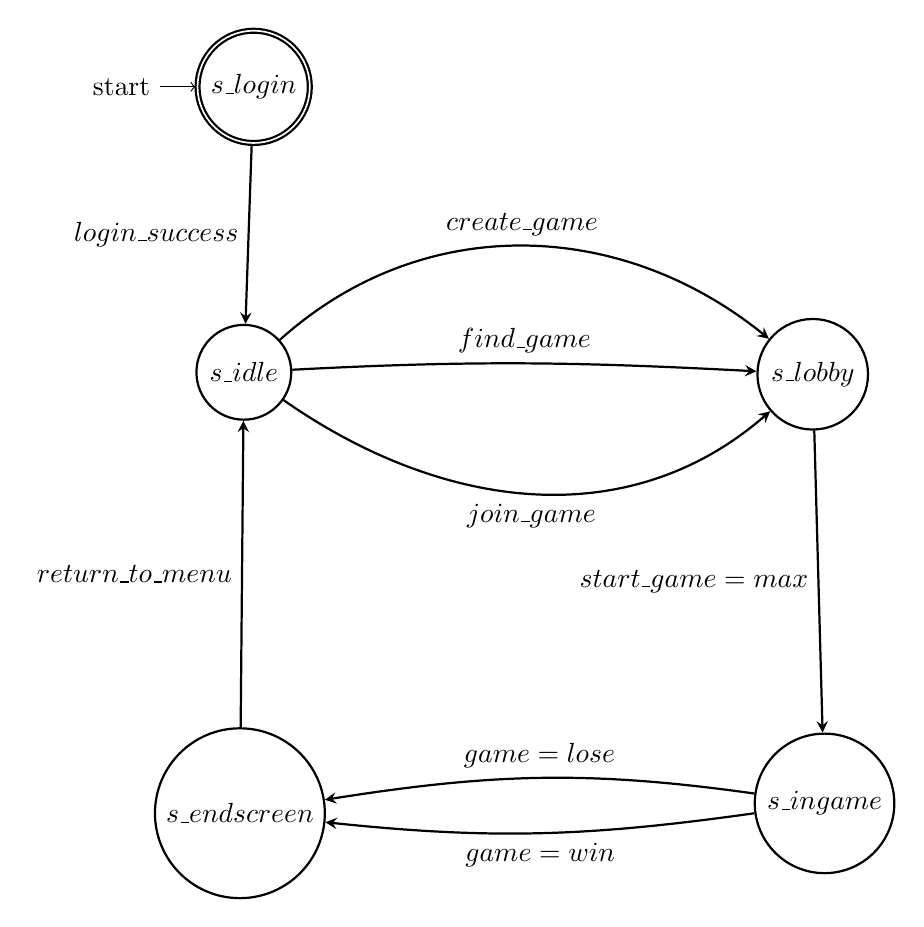
\begin{tikzpicture}[]
    \node[initial,thick,accepting,state] at (-3.9,4.175) (2a413fb1) {$s\_login$};
    \node[thick,state] at (-4.025,0.55) (e39a07c9) {$s\_idle$};
    \node[thick,state] at (3.2,0.525) (981cc1fb) {$s\_lobby$};
    \node[thick,state] at (3.35,-4.925) (d4f7f4ce) {$s\_ingame$};
    \node[thick,state] at (-4.075,-5.05) (21148f7e) {$s\_endscreen$};
    \path[->, thick, >=stealth]
    (2a413fb1) edge [left] node {$login\_success$} (e39a07c9)
    (e39a07c9) edge [above,in = 141, out = 42] node {$create\_game$} (981cc1fb)
    (e39a07c9) edge [above,in = 177, out = 3] node {$find\_game$} (981cc1fb)
    (e39a07c9) edge [below,in = -139, out = -35] node {$join\_game$} (981cc1fb)
    (981cc1fb) edge [left] node {$start\_game=max$} (d4f7f4ce)
    (d4f7f4ce) edge [above,in = 9, out = 172] node {$game=lose$} (21148f7e)
    (d4f7f4ce) edge [below,in = -6, out = -172] node {$game=win$} (21148f7e)
    (21148f7e) edge [left] node {$return\_to\_menu$} (e39a07c9)
    ;
\end{tikzpicture}
    \caption{Diagram for User State Finite State Machine}
    \label{fig:sm}
\end{figure}

\subsubsection{State Machine Definition}

Notation is based on standard academic conventions \cite{statemachine}.

$
\\
Let \, M = (Q, \Sigma, \delta, s, F)\\
Q = \{
    s\_login, s\_idle, s\_lobby, s\_ingame, s\_endscreen
\}\\
\sigma = \{
    login\_success, return\_to\_menu, create\_game,\\
    find\_game, join\_game, lobby\_size=max, game=lose, game=win
\}\\
\delta = \textrm{Shown in Figure \ref{fig:sm}}\\
s = s\_login\\
F = \{s\_login\}$




\subsection{Phase In Plan}

Functional requirements identified as priority level 0 are requirements which are integral to showcasing a proof of concept. The competition of these requirements sets a basis for the system, as many of these are needed for lower priority requirements. Additionally, they help identify the risks associated with the system and can help the developers understand if the planned solutions will work or not, as well as help in identifying missing requirements. On the other hand, competition of priority level 1 requirements will indicate the completion of a minimum viable product. The product can essentially be considered complete at this stage, which will allow for user acceptance testing to ensure that the product works for the end users. Finally, priority level 2 requirements encompass stretch goals which can improve the platform but are considered non-essential.

\begin{table}[h]
\begin{center}
\begin{tabular}{|c|c|}
\hline
    Priority Level & Date \\
    \hline
    0 & Nov 14th 2022 \\
    1 & Jan 7th 2022 \\
    2 & March 10th 2022 \\
    \hline
\end{tabular}
\end{center}
\caption{Phase In Plan for Functional Requirements}            

\end{table}


\section{Non-functional Requirements}

This section details the non-functional requirements of CodeChamp. Additionally, a fit criterion is specified alongside each non-functional requirement.


\subsection{Look and Feel Requirements}
\begin{enumerate}[label=NFR.\arabic*]
    \item All interactive elements shall provide feedback for the user. \label{NFR.1}
    \\\textbf{Fit Criterion}: Interact-able elements must have a hover effect upon mouse over events.
\end{enumerate}

\subsection{Usability and Humanity Requirements}
\begin{enumerate}[label=NFR.\arabic*, resume]
    \item All text displayed by the system should be readable.
    \\\textbf{Fit Criterion}: Text elements must have a color contrast ratio of at least 4.5:1 with the foreground element.
    \label{NFR.2}
    \item The system shall be simple to understand. \label{NFR.3}
    \\\textbf{Fit Criterion}: No more than 4 different options will be given to the user at a time.
\end{enumerate}
\subsection{Performance Requirements}
\begin{enumerate}[label=NFR.\arabic*, resume]
    \item The system's average response time will be 2 seconds or less. \label{NFR.4}
    \\\textbf{Fit Criterion}: The monthly average of all system responses must have an average response time of at most 2 seconds.
    \item The system's up-time percentage will be at least 99\%.
    \\\textbf{Fit Criterion}: The monthly system up-time must have an up time of 99\%.
    \label{NFR.5}
\end{enumerate}
\subsection{Operational and Environmental Requirements}
\begin{enumerate}[label=NFR.\arabic*, resume]
    \item The system should run on major browsers. \label{NFR.6}
    \\\textbf{Fit Criterion}: All parts of the system can be accessed and used by Google Chrome, Mozilla Firefox, Safari, Opera and Microsoft Edge's long term support versions as of February 2023.
\end{enumerate}
\subsection{Maintainability and Support Requirements}
N/A
\subsection{Security Requirements}
\begin{enumerate}[label=NFR.\arabic*, resume]
    \item The system shall deny the user access if the user is not logged in. \label{NFR.7}
    \\\textbf{Fit Criterion}: Unauthorized users must be redirected to login.
    \item The system shall prevent user code from accessing the file system.\label{NFR.8}
    \\\textbf{Fit Criterion}: Users must not give user access to the file system.
    \item The system shall prevent user code from making network calls.\label{NFR.9}
     \\\textbf{Fit Criterion}: Users' code with network calls is blocked from making network calls.
    \item The system shall run users' code in an isolated environment.\label{NFR.10}
    \\\textbf{Fit Criterion}: Users' code cannot access the system's environment.
\end{enumerate}
\subsection{Cultural Requirements}
\begin{enumerate}[label=NFR.\arabic*, resume]
    \item The system shall not have anything that is or suggests cultural inappropriate content to society. \label{NFR.11}
    \\\textbf{Fit Criterion}: None of the users involved in user acceptance testing should find any content that contains or implies anything that's culturally inappropriate.
\end{enumerate}
\subsection{Legal Requirements}
\begin{enumerate}[label=NFR.\arabic*, resume]
    \item The system shall be protected by the GNU General Public License (GPL). \label{NFR.12}
    \\\textbf{Fit Criterion}: All code for the CodeChamp system is accompanied by the GNU License.
\end{enumerate}
\subsection{Health and Safety Requirements}
\begin{enumerate}[label=NFR.\arabic*, resume]
    \item The system shall not have any flashing lights that can put the user under the risk of epilepsy or seizure. \label{NFR.13}
    \\\textbf{Fit Criterion}: All visuals must have no flashing lights.
\end{enumerate}
% This section is not in the original Volere template, but health and safety are
% issues that should be considered for every engineering project.


\section{Traceability}
% \begin{table}[H]
%     \begin{tabularx}{\textwidth}{|p{3cm}|p{3cm}|X|}
%     \hline
%     Non-Functional Requirements & Functional Requirements & Rationale \\
%     \hline
%     \ref{NFR.1}  & \ref{FR.4} \ref{FR.8} \ref{FR.14} \ref{FR.21} \ref{FR.22} \ref{FR.23} \ref{FR.24} & Requirements that are focused on interface design requirements.\\
%     \hline
%     \ref{NFR.2}  & \ref{FR.4} \ref{FR.8} \ref{FR.14} \ref{FR.21} \ref{FR.22} \ref{FR.23} \ref{FR.24} & Requirements that are focused on interface design requirements.\\
%     \hline
%     \ref{NFR.12} & \ref{FR.4} \ref{FR.8} \ref{FR.14} \ref{FR.21} \ref{FR.22} \ref{FR.23} \ref{FR.24} & Requirements that are focused on interface design requirements.\\
%     \hline
%     \ref{NFR.4} \ref{NFR.5} \ref{NFR.6} & \ref{FR.6} \ref{FR.7} \ref{FR.15} \ref{FR.16} \ref{FR.17} & Requirements that are focused on performance of user experience and code compilation.  \\
%     \hline
%     \ref{NFR.7} \ref{NFR.8}  \ref{NFR.9}& \ref{FR.17} \ref{FR.18} \ref{FR.19} & Requirements that are focused on account security and management\\
%     \hline
%     \end{tabularx}
%     \caption{Traceability Table for Functional and Non-Functional Requirements}
%     \label{tab:trace}
% \end{table}

\begin{landscape}
\begin{table}\begin{tabularx}{1.63\textwidth}{|p{1.1cm}|p{1.1cm}|p{1.1cm}|p{1.1cm}|p{1.1cm}|p{1.1cm}|p{1.1cm}|p{1.1cm}|p{1.1cm}|p{1.1cm}|p{1.3cm}|p{1.3cm}|p{1.3cm}|p{1.3cm}|}
    
    \hline
    & \ref{NFR.1} &\ref{NFR.2} & \ref{NFR.3} & \ref{NFR.4} & \ref{NFR.5} & \ref{NFR.6} & \ref{NFR.7} & \ref{NFR.8} & \ref{NFR.9} & \ref{NFR.10} & \ref{NFR.11} & \ref{NFR.12} & \ref{NFR.13}\\
    \hline
  \ref{FR.1} &  &  & & & & & & & & & & &\\\hline
  \ref{FR.2} &  & & X & & & & & & & & & &\\\hline
  \ref{FR.3} &  & & & & & & & & & & & &\\\hline
  \ref{FR.4} &  X & X & X & & & & & & & & & X & X \\\hline
  \ref{FR.5} &  & & X & & & & & & & & X & &\\\hline
  \ref{FR.6} &  & & & X & X & X & & & & X & & &\\\hline
  \ref{FR.7} &  & & & X & X & X & & & & X & & &\\\hline
  \ref{FR.8} & X & X & & & & & & & & &X & & X \\\hline
  \ref{FR.9} &  & & & & & & & & & & & &\\\hline
  \ref{FR.10} &  & & & & & & & & & & & &\\\hline
  \ref{FR.11} &  & & & & & & & & & & & &\\\hline
  \ref{FR.12} &  & & & & & & & & & & & &\\\hline
  \ref{FR.13} &  & & X & & & & & & & & & &\\\hline
  \ref{FR.14} & X & X & X & & & & & & & &X & & X\\\hline
  \ref{FR.15} &  & & & X & X & X & & & & X & & &\\\hline
  \ref{FR.16} &  & & & X & X & X & & & & X & & &\\\hline
  \ref{FR.17} &  & & & X & X & X & X & X & & & X & &\\\hline
  \ref{FR.18} &  & & X & & & & X & X & X & & X & &\\\hline
  \ref{FR.19} &  & & X & & & & X & X & X & & X & &\\\hline
  \ref{FR.20} &  & & X & & & & & & & & X & &\\\hline
  \ref{FR.21} & X & X & X & & & & & & & &X & & X \\\hline
  \ref{FR.22} & X & X & X & & & & & & & &X & & X \\\hline
  \ref{FR.23} & X & X & X & & & & & & & &X & & X\\\hline
  \ref{FR.24} & X & X & X & & & & & & & &X & & X \\\hline
  \end{tabularx}
    \caption{Traceability Matrix for Functional and Non-Functional Requirements}
    \label{tab:trace2}
\end{table}
\end{landscape} 

\section{Project Issues}

This section describes extra details regarding CodeChamp. This includes potential issues, the existing solutions, potential tasks, risks and costs of CodeChamp.

\subsection{Open Issues}
A critical part of the CodeChamp system involves compiling and executing user code, which can potentially be destructive to the system's security. As such, judging and evaluating a user submission and safely managing potentially malicious code are open issues which play an integral part in the success of the system.

\subsection{Off-the-Shelf Solutions}
There are several platforms which seek to address the same problem as CodeChamp. These platforms include LeetCode\cite{leetcode} and CodeForces\cite{codeforces}, which are problem repositories designed to help users practice algorithms and data structures. Unlike these platforms, CodeChamp introduces a guided process to eliminate the burden of searching for problems on the user's end. Additionally, CodeChamp will make the process fun and collaborative by allowing you to learn alongside friends and compete against others.

\subsection{New Problems}
As a competitive platform, CodeChamp will have to ensure that it is able to navigate the user through matches that are appropriate for their skill level. Additionally, it is important that users feel that they are challenged but not to an unfair extent, so the system should also match users with other players of an appropriate skill level.

\subsection{Tasks}
The back-end architecture must be designed to accommodate for all functional and non-functional requirements. Similarly, schemas need to be designed for the storage of data such as problems and user statistics in the database. Moreover, a user interface needs to be drafted and reviewed by potential users. Also, a communication schema needs to be decided between the front-end and back-end to allow for multiple concurrent connections. Finally, a verification and validation plan should be drafted and followed after the competition of an initial version of the product. The verification and validation effort should include plans for user acceptance testing, as well as functional and automated testing to ensure that the platform works as intended.

\subsection{Migration to the New Product}
N/A

\subsection{Risks}
A primary risk in the development of the CodeChamp system is its ability to handle multiple concurrent communications. Since our system aims to be a collaborative platform, many users will be using the system to compile and execute code, which can use a large amount of resources. Additionally the system should be able to protect itself from malicious use cases such as potential code injections and distributed denial-of-service attacks.

\subsection{Costs}
The primary costs for the platform will be back-end and front-end hosting server costs. Additionally, there will be costs associated with hosting a live-database for storage of data such as problems and user stats.

\subsection{User Documentation and Training}
N/A

\subsection{Waiting Room}
N/A

\subsection{Ideas for Solutions}
For concurrent communications and concurrent code compilations, vertical scaling for hardware is an easy fast method to remove the limitations of concurrency. However this leads to future higher costs. Load balancing can be used to allow for horizontal scaling of system.

For costs, many options exists for free/hobby tier project hosting, allowing for cost savings.

\newpage

\section{Appendix}

%This section has been added to the Volere template.  This is where you can place
%additional information.

\subsection{Identifying Required Knowledge}

What knowledge and skills will the team collectively need to acquire to successfully complete this capstone project? Examples of possible knowledge to acquire include domain-specific knowledge from the domain of your application, software engineering knowledge, mechatronics knowledge or computer science knowledge. Skills may be related to technology, writing, presentation, team management, etc. You should look to identify at least one item for each team member.

\begin{enumerate}

\item  \textbf{Presentation}:
Learning how to speak confidently in front of an audience allows for the best demonstration of our project. As we present our capstone, presentation skills will allow the team to reduce miscommunication and fully get our message across. Not only will this benefit the capstone project, it is a transferable skill to the real world. 

\item  \textbf{Project Management}:
Project management for a team of 5 with a large project isn't something the team is familiar with and it is key for completing our project successfully. This includes splitting off features/work among us, reviewing each other's pull requests and planning meetings or sprints.

\item \textbf{Two way web communication technology}: Learning this technology will be necessary for the success of our project as it is required to make our project collaborative. This technology will allow the project to communication between server and client and will be a key part of our project.

\item  \textbf{Continuous Integration and Continuous Delivery (CI/CD) - Zhiming Zhao}:
CI/CD connects development and operation activities together, it will enforce automation in developing, building, testing and code deployment. CI/CD compiles the incremental code changes made by developers, then package them as software deliverable. Automated tests are running constantly to verify the software functionality, and automated deployment services deliver them to end users. 

\item \textbf{System Design - Youssef Rizkalla}: 
Architecting a good design for the back-end and front-end of the system is essentially to creating a friction-less environment that allows us to fulfill and test the requirements according to their deadlines. Learning design patterns and applying them when needed will be necessary, as well as learning how to enforce coding standards when reviewing and writing code to maintain codebase health.

\end{enumerate}

\subsection{Acquiring Required Knowledge}

For each of the knowledge areas and skills identified in the previous question, what are at least two approaches to acquiring the knowledge or mastering the skill? From the identified approaches, which will each team member pursue, and why did they make this choice?

\begin{enumerate}

\item \textbf{Presentation - Dipendra Subedi} An approach to develop presentation skills is to practice speaking in front of audiences. In front of an audience, we can increase the confidence for public speaking, practice maintaining eye-contact, and speaking coherently. Another approach is to participate as a member of the audience in a presentation with great speakers. Being able to mimic exemplary presentation skills can be a guide when we are presenting ourselves. Dipendra will work on this skill as he is the design lead, so it is crucial to be able to effectively communicate ideas. When presenting the capstone project, this will also help since he will take more of a speaking role to describe the system.

\item  \textbf{Project Management - Tamas Leung}: In order to learn project management is through researching and testing out different project management strategies. This involves learning tools such as GitHub project board/kanban boards. This can be practiced by assigning priorities and weights to tasks and ensuring other teammates have a good weight of tasks per week. Tamas will work on this skill as he is the scrum lead. He will ensure that every task is on a timeline and are on track to be finished as stated on the development plan.

\item \textbf{Two way web communication technology - Anton Kanugalawattage}: This skill could be acquired by reading and following examples of existing implementation using this technology. Another approach to acquire this skill is to read the documentation or blogs of how this technology is used in systems (networking classes, technology company's engineering blogs). Anton will pursue this skill as he has worked on a project which has utilized a similar technology before. Also, as he is the front-end lead this technology will be a crucial part of the front-end and back-end integration. 

\item \textbf{CI/CD - Zhiming Zhao}: There are a lot of benefits to adapt CI/CD. First of all, there will be reduced risk on delivery. The automated tests will test the code changes before it's deployed, this will result in a higher product quality and low rates of bugs in production. The software will ship quickly and more efficiently since CI/CD pipelines move applications from coding to deployment at scale. The team will also have improved productivity since everything is moving at a faster pace.

\item\textbf{System Design - Youssef Rizkalla}: This can be developed by observing and critiquing open-source projects, as well as projects previously worked on. Youssef will work on this as he is the back-end lead and main code-reviewer. By doing this, he can identify issues that have occurred in the past and develop a design to get around them. Additionally, design patterns can be learned from official documentation or trustworthy blog posts that are published by professional Software Engineers. When reviewing code, Youssef can ensure that others are following the correct standards and design patterns. Additionally, re-iterations of the design can be done as needed if engineers feel that features are taking longer to develop and/or test than they should be.

\end{enumerate}

\subsection{Symbolic Parameters}
N/A
%The definition of the requirements will likely call for SYMBOLIC\_CONSTANTS.
%Their values are defined in this section for easy maintenance.


\begin{thebibliography}{9}
\bibitem{statemachine}
N.R. Satish, University of California, Berkeley. (n.d.). Finite State Machine. Our Pattern Language. Retrieved October 3, 2022, from \href{https://patterns.eecs.berkeley.edu/?page_id=470}{https://patterns.eecs.berkeley.edu/?page\_id=470} 

\bibitem{leetcode}
The world's leading online programming learning platform. LeetCode. (n.d.). Retrieved March 30, 2023, from \href{from https://leetcode.com/}{https://leetcode.com/} 

\bibitem{codeforces}
Codeforces. (n.d.). Retrieved March 30, 2023, from  \href{https://codeforces.com/}{https://codeforces.com/} 
\end{thebibliography}

\end{document}
